\uuid{fN7t}
\exo7id{5915}
\titre{exo7 5915}
\auteur{rouget}
\organisation{exo7}
\datecreate{2010-10-16}
\isIndication{false}
\isCorrection{true}
\chapitre{Surfaces}
\sousChapitre{Plan tangent, vecteur normal}
\module{Géométrie}
\niveau{L2}
\difficulte{}

\contenu{
\texte{
Soit $\mathcal{S}$ la surface d'équation $x^4-x^3+xy-y^2-z=0$.
}
\begin{enumerate}
    \item \question{Déterminer les plans tangents à la surface $\mathcal{S}$ parallèle au plan $\left(O,\overrightarrow{i},\overrightarrow{j}\right)$.}
\reponse{Pour $(x,y)\in\Rr^2$, posons $f(x,y)=x^4-x^3+xy-y^2$ puis pour $(x,y,z)\in\Rr^3$, posons $g(x,y,z)=z-f(x,y)$. $\mathcal{S}$ est la surface d'équation $z=f(x,y)$ ou encore $g(x,y,z)=0$.

La fonction $g$ est de classe $C^1$ sur $\Rr^3$ et pour tout $(x,y,z)\in\Rr^3$,

\begin{center}
$\left(\overrightarrow{\text{grad}}\;g\right)(x,y,z)=\left(
\begin{array}{c}
- \frac{\partial f}{\partial x}(x,y)\\
\rule[-4mm]{0mm}{11mm}- \frac{\partial f}{\partial y}(x,y)\\
1
\end{array}
\right)=\left(
\begin{array}{c}
-4x^3+3x^2-y\\
-x+2y\\
1
\end{array}
\right)\neq\overrightarrow{0}$.
\end{center}

Donc, la surface $\mathcal{S}$ est régulière et en tout point $(x_0,y_0,z_0)$ de la surface $\mathcal{S}$, le vecteur gradient est un vecteur normal au plan tangent $\mathcal{P}_0$ à la surface $\mathcal{S}$ en $(x_0,y_0,z_0)$. Le plan 

\begin{align*}\ensuremath
\mathcal{P}_0\;\text{parallèle à}\;\left(O,\overrightarrow{i},\overrightarrow{j}\right)&\Leftrightarrow\left\{
\begin{array}{l}
-4x_0^3+3x_0^2-y_0=0\\
-x_0+2y_0=0
\end{array}
\right.\Leftrightarrow\left\{
\begin{array}{l}
x_0=2y_0\\
-y_0(32y_0^2-12y_0+1)=0
\end{array}
\right.\Leftrightarrow\left\{
\begin{array}{l}
x_0=2y_0\\
-y_0(32y_0^2-12y_0+1)=0
\end{array}
\right.
\\
 &\Leftrightarrow y_0=0=x_0\;\text{ou}\;(y_0= \frac{1}{4}\;\text{et}\;x_0= \frac{1}{2})\;\text{ou}\;(y_0= \frac{1}{8}\;\text{et}\;x_0= \frac{1}{4})
\end{align*}

On obtient ainsi les trois points $O(0,0,0)$, $A\left( \frac{1}{2}, \frac{1}{4},0\right)$ et $B\left( \frac{1}{4}, \frac{1}{8}, \frac{1}{256}\right)$.}
    \item \question{Etudier localement la position relative de la surface $\mathcal{S}$ et de son plan tangent en chacun des points ainsi obtenu.}
\reponse{La fonction $f$ est de classe $C^2$ sur $\Rr^2$ et

\begin{center}
$rt-s^2= \frac{\partial^2}{\partial x^2} \frac{\partial^2}{\partial y^2}-\left( \frac{\partial^2}{\partial x\partial y}\right)^2=(12x^2-6x)(-2)-1^2=-24x^2+12x-1$
\end{center}

\textbullet~En $O$, le plan tangent est le plan $\left(O,\overrightarrow{i},\overrightarrow{j}\right)$. De plus, $(rt-s^2)(0,0)=-1<0$. Donc le point $O$ est un point selle.

\textbullet~En $A$, le plan tangent est aussi le plan $\left(O,\overrightarrow{i},\overrightarrow{j}\right)$. De plus, $(rt-s^2)\left( \frac{1}{2}, \frac{1}{4}\right)=-1<0$. Donc le point $A$ est un point selle.

\textbullet~En $B$, le plan tangent est le plan d'équation $z= \frac{1}{256}$. De plus, $(rt-s^2)\left( \frac{1}{4}, \frac{1}{8}\right)= \frac{1}{2}>0$. Donc la surface $\mathcal{S}$ a une disposition en ballon au point $B$.}
    \item \question{Etudier la position relative globale de la surface $\mathcal{S}$ et du plan $\left(O,\overrightarrow{i},\overrightarrow{j}\right)$.}
\reponse{Il s'agit maintenant d'étudier le signe de $z=f(x,y)=x^4-x^3+xy-y^2$ sur $\Rr^2$.

\begin{center}
$f(x,y)=x^4-x^3+xy-y^2=(x^4-y^2)-x(x^2-y)=(x^2-y)(x^2+y-x)$.
\end{center}

L'intersection de la surface $\mathcal{S}$ avec le plan $\left(O,\overrightarrow{i},\overrightarrow{j}\right)$ est donc la réunion des deux paraboles d'équations respectives $y=x^2$ et $y=-x^2+x$ dans le plan $\left(O,\overrightarrow{i},\overrightarrow{j}\right)$. Représentons cette intersection ainsi que le signe de $f(x,y)\oplus\ominus$.

$$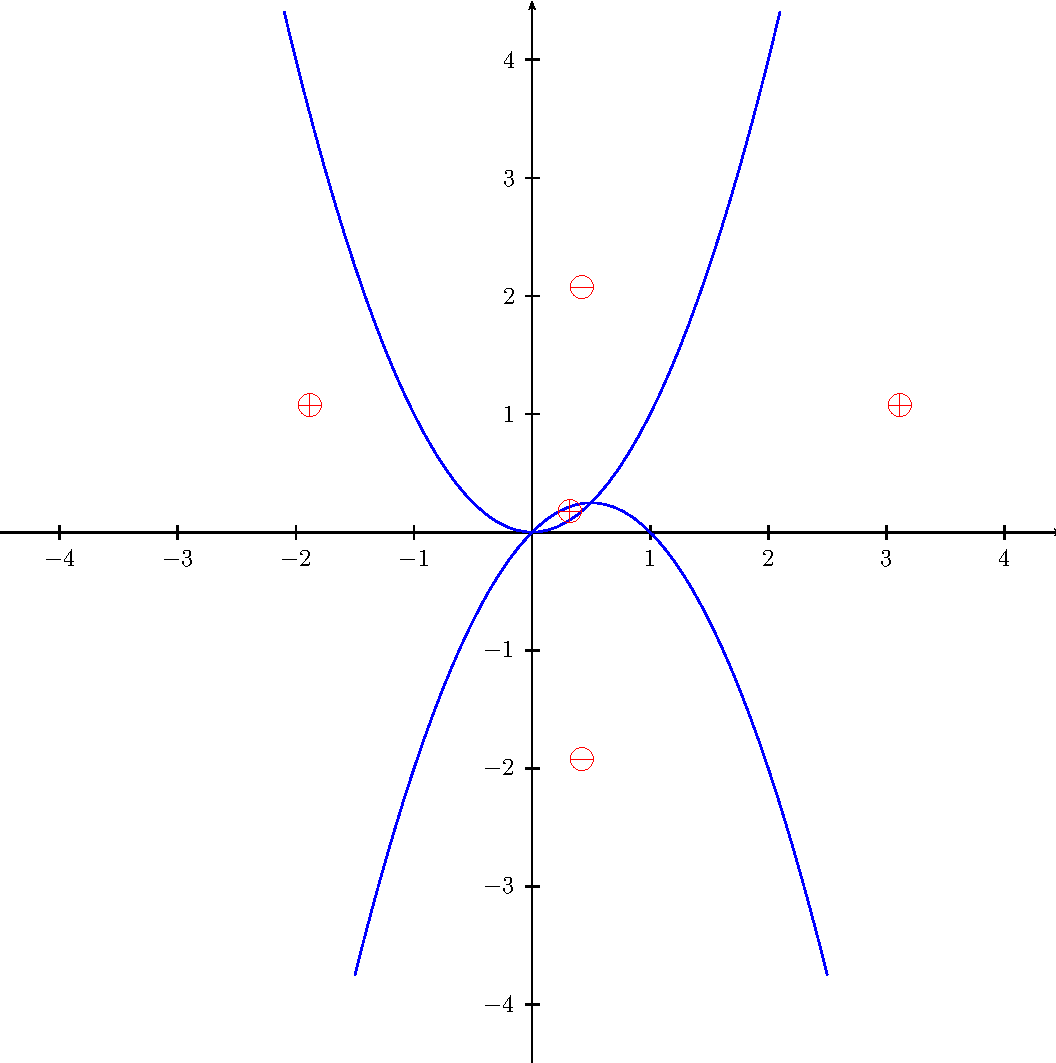
\includegraphics{../images/img005915-1}$$}
\end{enumerate}
}
